\paragraph{Menús} \hspace{1cm}\\ 
Las funcionalidades de la herramienta se encuentran organizadas por algunos menús. Cada usuario accede a diferentes menús en sus respectivas aplicaciones con las funciones que cada uno de ellos puede realizar.\\

\subparagraph{Menús aplicación Entrenador} \hspace{1cm}\\ 
La aplicación que corresponde al Entrenador contiene cuatro menús distintos, cada uno con funcionalidades propias. \\

\textbf{\textcolor[rgb]{0, 0, 0.545098}{Menú Entrenador}}\\

En la figura \ref{menu:ME01} se muestran las opciones del menú principal que serán visibles para el actor Entrenador. Las opciones del menú se enlistan a continuación:\\

\begin{compactitem} 
	\setlength\itemsep{-0.25em}
	\item Practicantes
	\item Captura
	\item Rutinas
\end{compactitem} 

\begin{figure}[H]
	\centering
		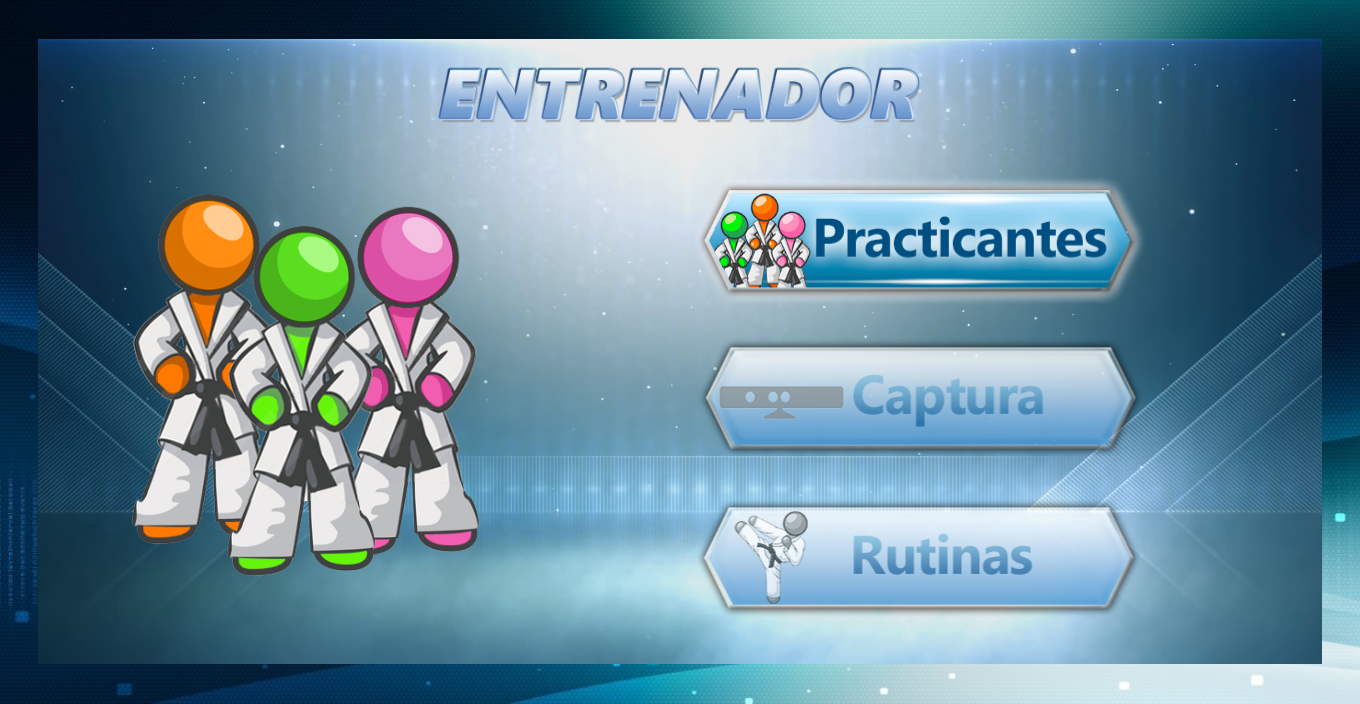
\includegraphics[scale=0.5]{./Figuras/Menus/ME01Menu_Entrenador}
	\caption{ME01 Menú Entrenador}
	\label{menu:ME01}
\end{figure}

\textbf{\textcolor[rgb]{0, 0, 0.545098}{Menú Practicantes}}\\

Al seleccionar la opción "Practicantes" se mostrará un nuevo menú que se muestra en la figura \ref{menu:ME02} y con las opciones que se muestra a continuación:\\

\begin{compactitem} 
	\setlength\itemsep{-0.25em}
	\item Registrar Practicante
	\item Lista de Practicantes
\end{compactitem} 

\begin{figure}[H]
	\centering
		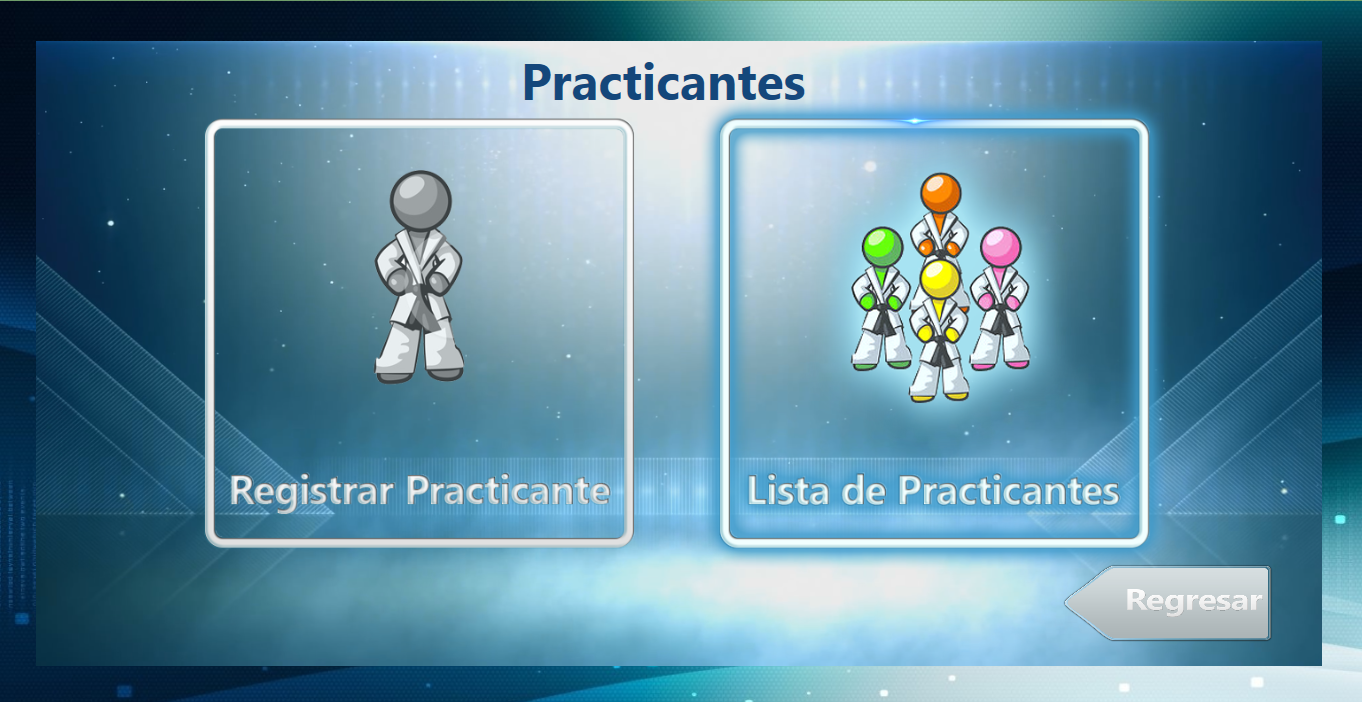
\includegraphics[scale=0.5]{./Figuras/Menus/ME02Practicantes}
	\caption{ME02 Menú Practicantes}
	\label{menu:ME02}
\end{figure}

\textbf{\textcolor[rgb]{0, 0, 0.545098}{Menú gestionar rutinas}}\\

En la figura \ref{menu:ME03} se muestran las opciones del menú para gestionar las rutinas de entrenamiento. Las opciones del menú se enlistan a continuación:\\

\begin{compactitem} 
	\setlength\itemsep{-0.25em}
	\item Modificar Rutina
	\item Eliminar Rutina
\end{compactitem} 

\begin{figure}[H]
	\centering
		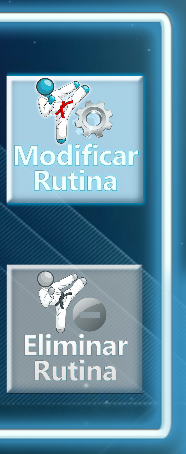
\includegraphics[scale=0.5]{./Figuras/Menus/ME03Gestionar_rutinas}
	\caption{ME03 Menú gestionar rutinas}
	\label{menu:ME03}
\end{figure}

\textbf{\textcolor[rgb]{0, 0, 0.545098}{Menú gestionar Practicantes}}\\

En la figura \ref{menu:ME04} se muestran las opciones del menú para gestionar a los Practicantes registrados en la herramienta. Las opciones del menú se enlistan a continuación:\\

\begin{compactitem} 
	\setlength\itemsep{-0.25em}
	\item Modificar Información
	\item Asignar Rutina
	\item Visualizar Indicadores
	\item Dar de baja Practicante
\end{compactitem} 

\begin{figure}[H]
	\centering
		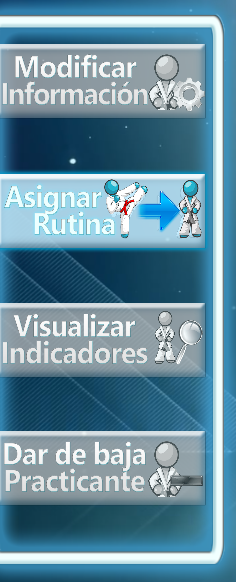
\includegraphics[scale=0.5]{./Figuras/Menus/ME04Gestionar_Practicantes}
	\caption{ME04 Menú gestionar Practicantes}
	\label{menu:ME04}
\end{figure}

\subparagraph{Menús aplicación Practicante} \hspace{1cm}\\ 
La aplicación que corresponde al Practicante contiene dos menús distintos, cada uno con funcionalidades propias. \\

\textbf{\textcolor[rgb]{0, 0, 0.545098}{Menú Practicante}} \\

En la figura \ref{menu:MP01} se muestran las opciones del menú principal que serán visibles para el actor Practicante. Las opciones del menú se enlistan a continuación:\\

\begin{compactitem} 
	\setlength\itemsep{-0.25em}
	\item Datos Personales
	\item Lista de Rutinas
	\item Lista de Comentarios
	\item Cerrar Sesión.
\end{compactitem}

\begin{figure}[H]
	\centering
		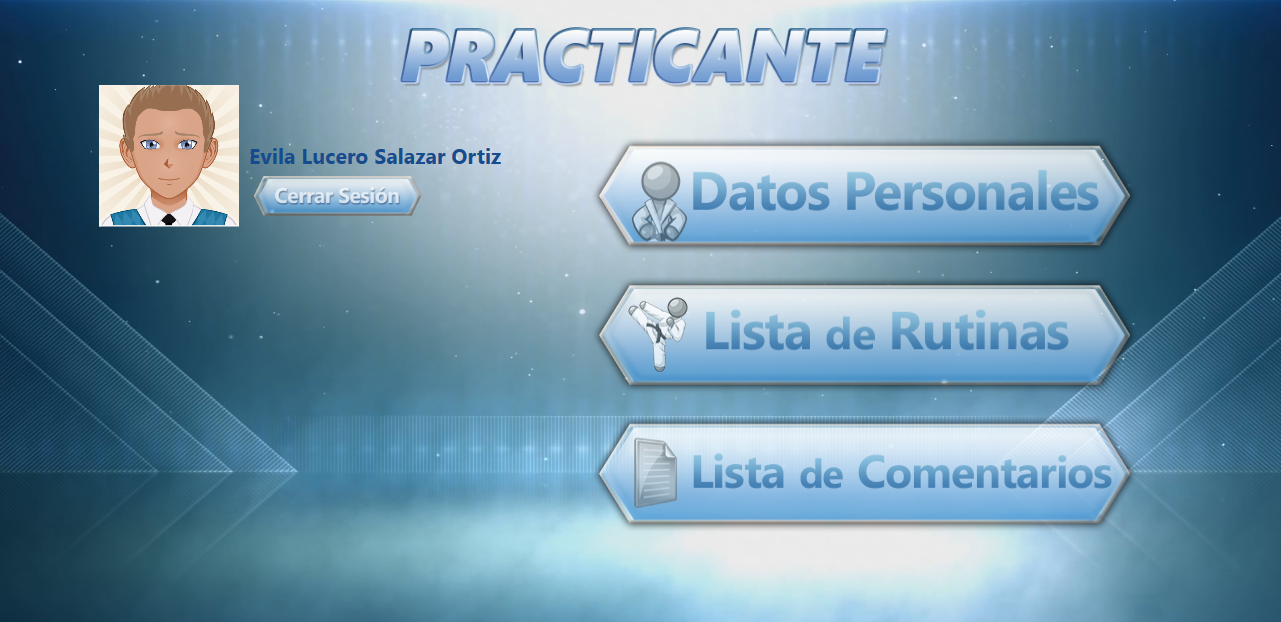
\includegraphics[scale=0.5]{./Figuras/Menus/MP01Menu_Practicante}
	\caption{MP01 Menú Practicante}
	\label{menu:MP01}
\end{figure}
	
\textbf{\textcolor[rgb]{0, 0, 0.545098}{Menú de rutinas}} \\

En la figura \ref{menu:MP02} se muestran las opciones del menú de las rutinas de entrenamiento que el Entrenador le ha asignado al Practicante. Las opciones del menú se enlistan a continuación: \\

\begin{compactitem} 
	\setlength\itemsep{-0.25em}
	\item Realizar Rutina
	\item Enviar Rutina
\end{compactitem} 

\begin{figure}[H]
	\centering
		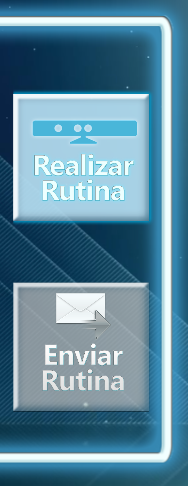
\includegraphics[scale=0.5]{./Figuras/Menus/MP02Menu_rutinas}
	\caption{MP02 Menú de rutinas}
	\label{menu:MP02}
\end{figure}

%\clearpage